% !TeX program = xelatex
\documentclass[UTF8,a4paper,11pt,fontset=windows]{ctexart}
\usepackage[margin=21mm]{geometry}
\usepackage{amsmath,amssymb,booktabs,graphicx,float,longtable,tikz,xcolor}
\usetikzlibrary{arrows.meta,positioning,calc}
\usepackage[colorlinks=true,linkcolor=blue!55!black,urlcolor=blue!55!black]{hyperref}
\setlength{\parskip}{0.4em}\setlength{\emergencystretch}{2em}
\setcounter{tocdepth}{1}
\newcommand{\file}[1]{\texttt{\detokenize{#1}}}
\newcommand{\Kfinal}{\frac{-21.5(s+0.136)(s+0.16)}{s(s+0.0015)(s+0.31)(s+10.7)(s+14.5)}}
\newcommand{\Gplant}{\frac{-88.196939s(s+4.704978)(s+0.06347365)}{D_a(s)}}

\title{AERO5560 Group 8\\俯仰角速度内环设计}
\author{Group 8}\date{2026年10月20日}
\begin{document}\maketitle
\begin{abstract}
针对约 200 节、300 ft 配平点比较三种俯仰角速度补偿器。最终闭环带宽为 4.237 rad/s，开环交越频率为 2.017 rad/s，调节时间 1.607 s，稳态误差 0.116\%，超调 8.897\%。验证包括邻近空速、假设舵机动态、参数扰动、非线性机动、测量噪声和数字实现。
\end{abstract}
\tableofcontents\clearpage
\section{要求与模型}
纵向 Task 1 要求提取 $G_{q\delta_e}$、绘制反馈框图，并比较至少三种补偿器，给出根轨迹、Bode 和阶跃响应。对 $4^\circ$/s 阶跃，要求调节时间不超过 3 s、稳态误差小于 1\%、超调小于 20\%、升降舵位于 $\pm25^\circ$ 内；频率目标为 2--10 rad/s，噪声带宽为 20 rad/s。

分别报告开环交越频率 $|L(j\omega_{gc})|=1$ 与闭环带宽 $|T(j\omega_{BW})|=10^{-3/20}|T(0)|$ [1,2]。调节时间同时按最终值和指令值的 $\pm2\%$ 范围计算，超调以最终值为基准。线性角速度指标检查 120 s，舵角极值检查前 10 s；非线性测试采用 5 s 阶跃，以及总仿真 10 s、持续 2 s 的脉冲。

Lecture 8-2 第 8 页及 Lecture 9-1 第 9、17 页采用噪声阈值处衰减 40 dB 的标准。20 rad/s 开环幅值为 $-41.390$ dB，闭环噪声传递为 $-41.409$ dB，均满足要求。20--$10^5$ rad/s 扫描确认整个检查频段的衰减至少为 40 dB。

\subsection{飞机参数与纵向动态}
飞机质量 750 kg、翼面积 11.9 m$^2$、弦长 0.85 m、俯仰惯量 1766.52 kg m$^2$。名义速度 102.888 m/s、高度 91.44 m，密度 1.21427 kg/m$^3$、动压 6427.1 Pa；配平油门 0.770317，升降舵 $+0.766074^\circ$。

固定高度模型采用 $[\Delta u,\Delta w,\Delta q,\Delta\theta]^T$，固定油门、零阵风。由收敛后的中心差分矩阵得到
\begin{align}
G(s)&=\Gplant,\\
D_a(s)&=(s+4.231362-j3.300400)(s+4.231362+j3.300400)\notag\\
&\quad\times(s+0.0303971-j0.0772921)(s+0.0303971+j0.0772921).
\end{align}
保留全部纵向模态。短周期固有频率为 5.36629 rad/s，阻尼比为 0.788508。

\section{带宽选择}
综合模态频率、舵效、噪声与执行机构响应，选择闭环带宽 4.237 rad/s，低于短周期固有频率。对应约化频率 $c\omega/(2V)=0.01750$，与 20 rad/s 噪声阈值保留频率间隔。

此前 6.707 rad/s 方案未满足噪声要求。新增高频极点并重新调整低频零极点后，带宽降低，跟踪指标保持达标。下表固定零极点、只改变增益，展示提高交越频率造成的噪声衰减减弱及稳定性损失。

\begin{table}[H]\centering\small\caption{只改变增益的频率取舍；频率单位 rad/s。}
\begin{tabular}{lrrrrr}\toprule
$\omega_{gc}$ & $\omega_{BW}$ & $t_s$ (s) & OS (\%) & PM (deg) & $|T(j20)|$ (dB)\\\midrule
2.00 & 4.20 & 1.61 & 8.54 & 60.59 & -41.48\\
3.00 & 5.63 & 2.82 & 28.78 & 43.35 & -37.87\\
4.00 & 6.61 & 5.12 & 49.57 & 25.35 & -34.88\\
$\infty$ & $\infty$ & $\infty$ & $\infty$ & $\infty$ & $\infty$\\
$\infty$ & $\infty$ & $\infty$ & $\infty$ & $\infty$ & $\infty$\\
$\infty$ & $\infty$ & $\infty$ & $\infty$ & $\infty$ & $\infty$\\
\bottomrule\end{tabular}\end{table}

\begin{figure}[H]\centering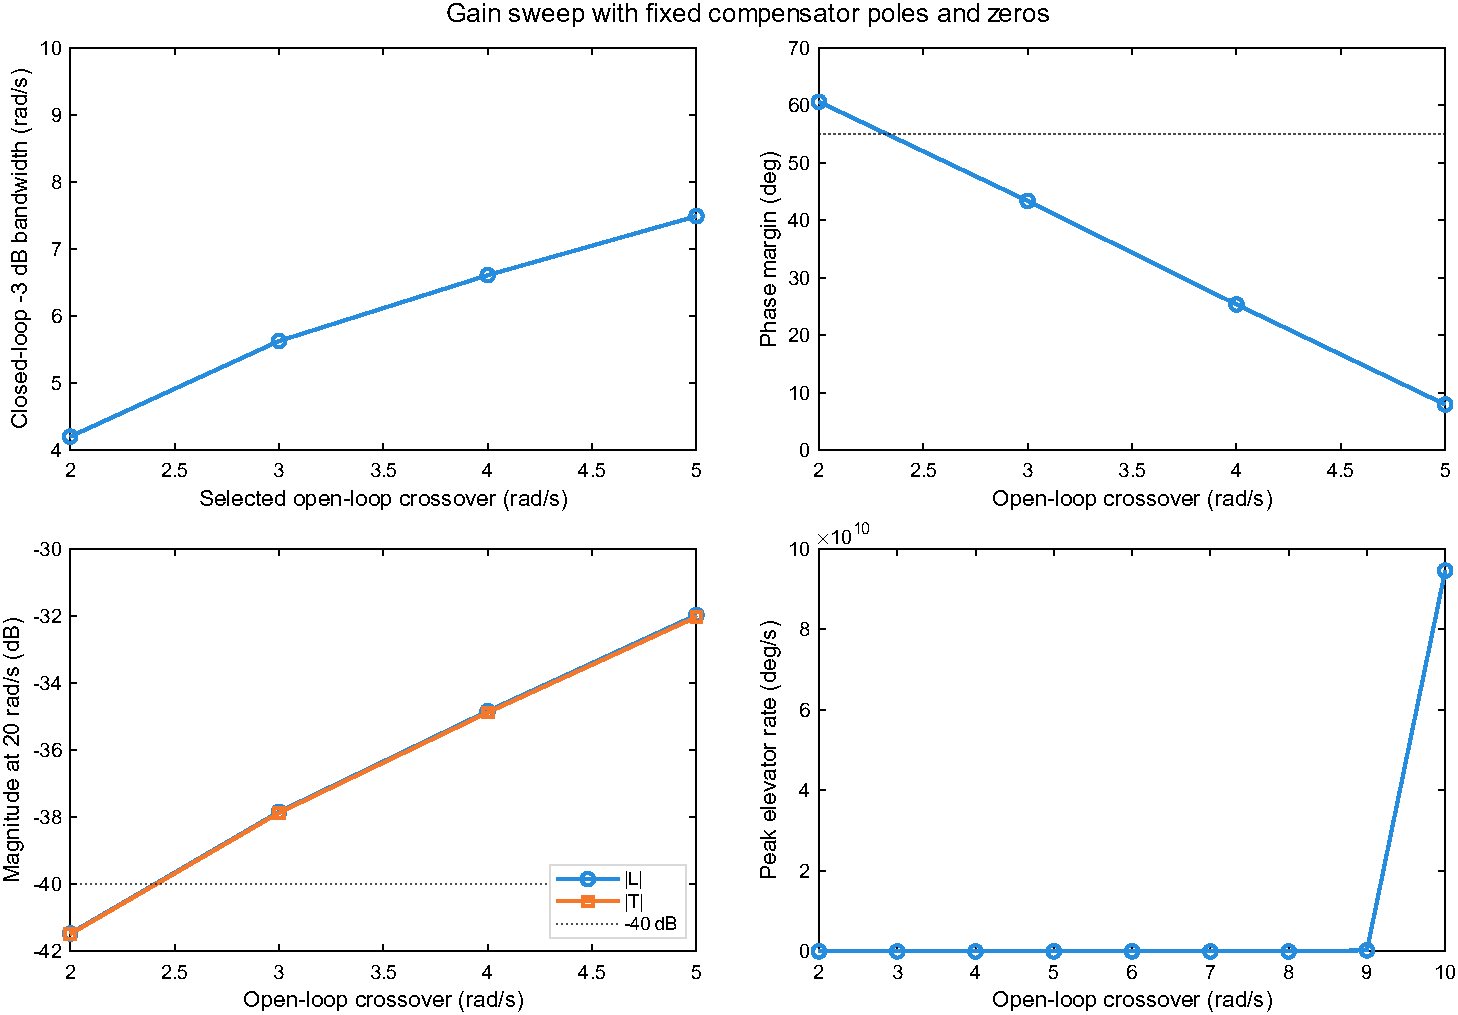
\includegraphics[width=1.0\linewidth]{frequency_trade.pdf}\caption{固定补偿器形状时的频率取舍。}\end{figure}

后续垂直速度外环可从 0.5--1 rad/s 开始设计，并检查串级系统的耦合稳定性。

\section{反馈与灵敏度函数}

\begin{figure}[H]\centering
\resizebox{\linewidth}{!}{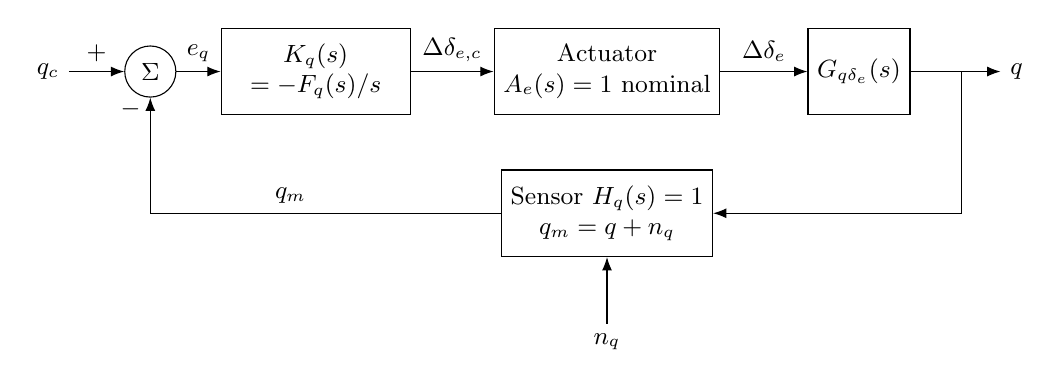
\begin{tikzpicture}[>=Latex,block/.style={draw,minimum height=1.1cm,align=center},font=\small]
\node (r) at (0,0) {$q_c$};
\node[draw,circle,minimum size=6mm] (sum) at (1.3,0) {$\Sigma$};
\node[block,minimum width=2.4cm] (k) at (3.4,0) {$K_q(s)$\\$=-F_q(s)/s$};
\node[block] (a) at (7.1,0) {Actuator\\$A_e(s)=1$ nominal};
\node[block] (g) at (10.3,0) {$G_{q\delta_e}(s)$};
\node (y) at (12.3,0) {$q$};
\draw[->](r)--node[above]{$+$}(sum);
\draw[->](sum)--node[above]{$e_q$}(k);
\draw[->](k)--node[above]{$\Delta\delta_{e,c}$}(a);
\draw[->](a)--node[above]{$\Delta\delta_e$}(g);
\draw[->](g)--(y);
\node[block] (h) at (7.1,-1.8) {Sensor $H_q(s)=1$\\$q_m=q+n_q$};
\draw[->](11.6,0)|-(h);
\draw[->](h)-|node[pos=.3,above]{$q_m$}(sum) node[pos=.95,left]{$-$};
\draw[->](7.1,-3.2)node[below]{$n_q$}--(h.south);
\end{tikzpicture}}
\caption{Pitch-rate feedback. Physical elevator is $\delta_{e0}+\Delta\delta_e$; nominal trim is $+0.766074^\circ$. All dynamic signals use rad and s.}
\end{figure}

飞机传递函数增益为负，因此控制器取负增益。SISOtool 使用
\begin{equation}
P_q=\operatorname{minreal}(-G/s),\qquad K_q=-F_q/s,\qquad L=P_qF_q=GK_q.
\end{equation}
按 Lecture 10-1，在外部加入一个积分器，抵消最小 q 通道的原点零点；工具中的 plant 为 $P_q$、compensator 为 $F_q$。控制器零极点均为实数，最终开环严格真有理。
\begin{equation}S=\frac{1}{1+L},\qquad T=\frac{L}{1+L}=1-S,\qquad U=K_qS.\end{equation}
指令到 q 为 $T$，到舵面为 $U$；测量噪声到 q 为 $-T$，到舵面为 $-U$。若 $d_e$、$d_q$ 分别作用于飞机输入和输出，则 $q=Tq_c+GSd_e+Sd_q-Tn_q$。$T$ 对应课程 SCK 中的互补灵敏度 $C$；数值 ZPK 见 \file{zpk.txt}。

低频时 $G\sim-132.596s$，原点抵消后的最小开环为 type 0：
\begin{equation}\frac{e_{ss}}{q_c}=\frac{1}{1+L(0)},\qquad L(0)>99\ \text{时误差小于 }1\%.\end{equation}
最终直流开环增益为 859.85，即 58.69 dB。滞后补偿提高低频增益，同时控制交越附近的增益。

\section{补偿器迭代}
\subsection{第一轮：积分增益}
\begin{equation}K_{q,1}(s)=-0.1961/s.\end{equation}
开环交越频率约 3 rad/s，但稳态误差为 3.70\%，慢尾部使调节时间达到 10.92 s，两项均需改进。
\begin{figure}[H]\centering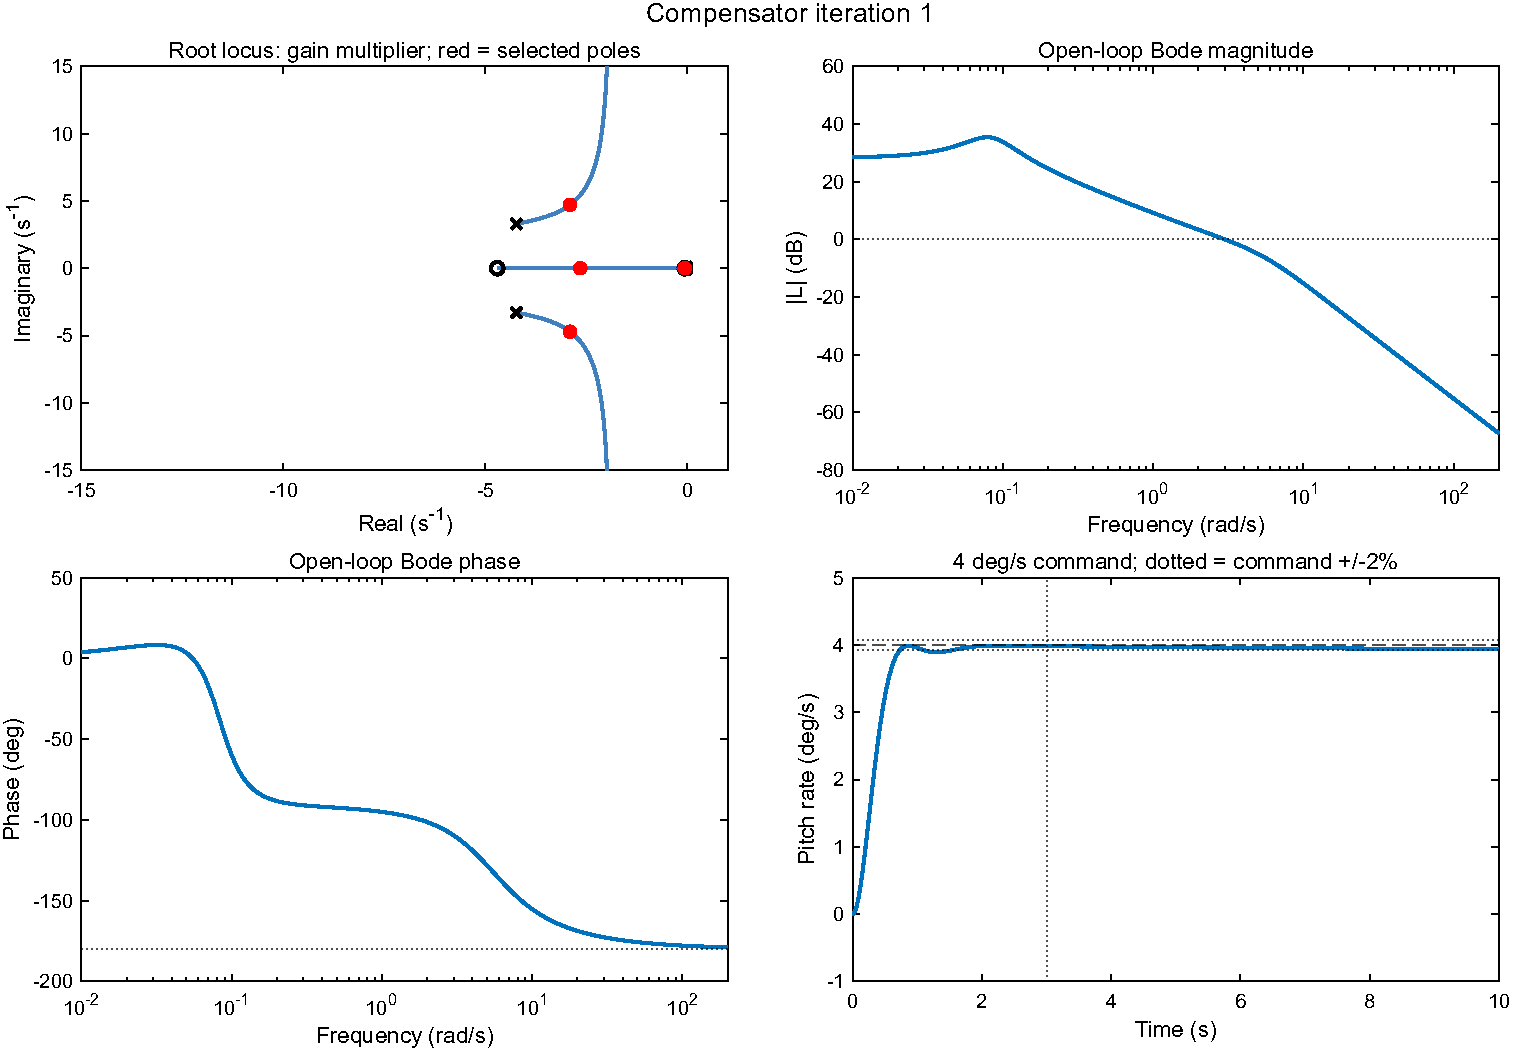
\includegraphics[width=1.0\linewidth]{iteration_1.pdf}\caption{第 1 轮：根轨迹局部、Bode 与 4 deg/s 阶跃；红点为选定闭环极点。}\end{figure}

\clearpage\subsection{第二轮：滞后与高频滚降}
\begin{equation}K_{q,2}(s)=\frac{-5.835(s+0.5)}{s(s+0.1)(s+30)}.\end{equation}
滞后零极点比为五，稳态误差降至 0.77\%，超调低于 20\%；相位损失与慢动态使调节时间仍有 4.55 s。
\begin{figure}[H]\centering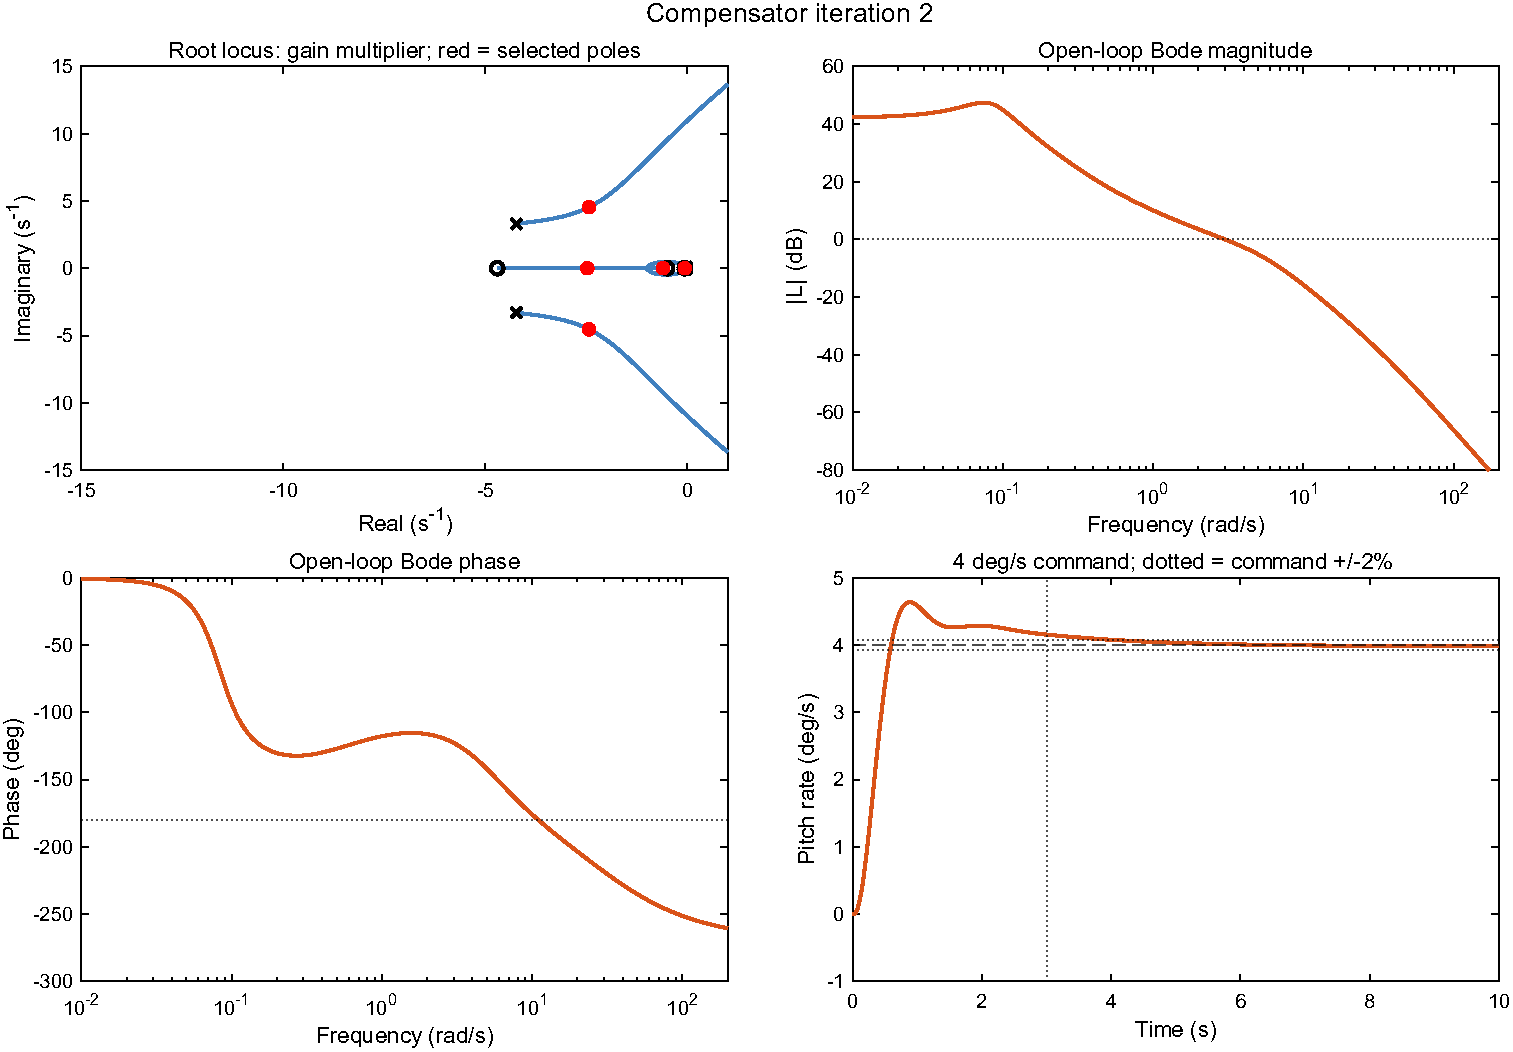
\includegraphics[width=1.0\linewidth]{iteration_2.pdf}\caption{第 2 轮：根轨迹局部、Bode 与 4 deg/s 阶跃；红点为选定闭环极点。}\end{figure}

\clearpage\subsection{第三轮：低频补偿与噪声滚降}
\begin{equation}\boxed{K_q(s)=\Kfinal.}\end{equation}
SISOtool 中的补偿器为
\begin{equation}F_q(s)=\frac{21.5(s+0.136)(s+0.16)}{(s+0.0015)(s+0.31)(s+10.7)(s+14.5)}.\end{equation}
低频补偿提高直流增益，10.7 与 14.5 rad/s 极点提供额外噪声滚降。原点抵消后开环为八极点、四零点。参数针对名义模型、重新配平的 180 节模型和假设的 50 ms 舵机调整，再简化、取整复核。
\begin{figure}[H]\centering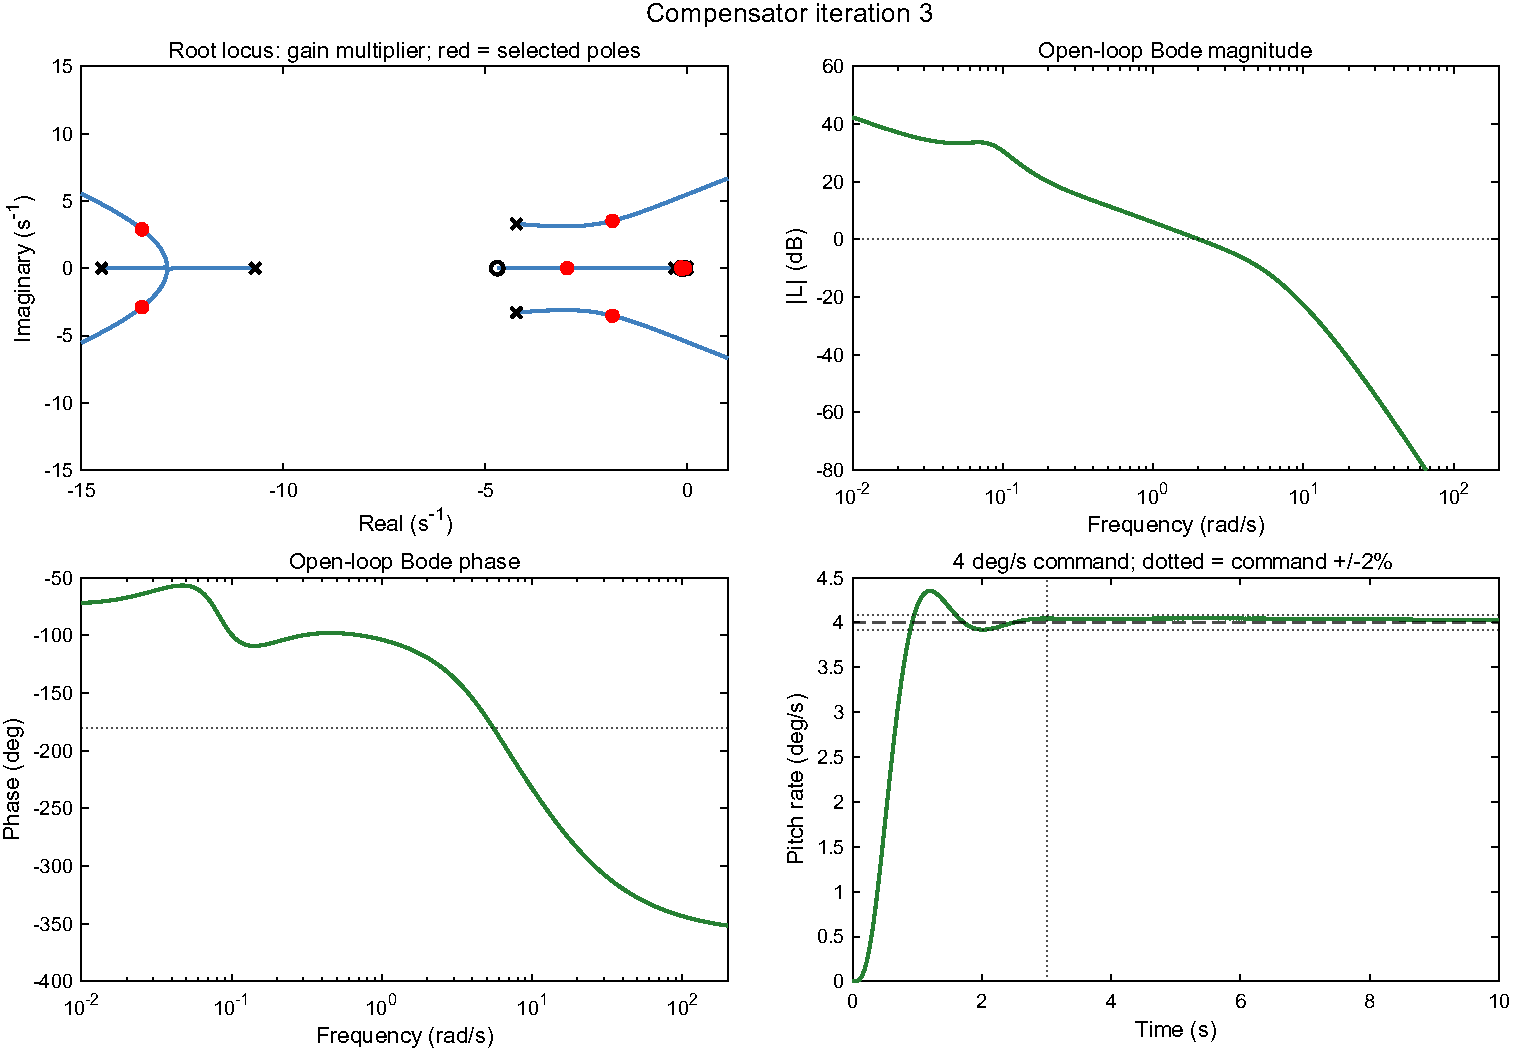
\includegraphics[width=1.0\linewidth]{iteration_3.pdf}\caption{第 3 轮：根轨迹局部、Bode 与 4 deg/s 阶跃；红点为选定闭环极点。}\end{figure}

\clearpage\subsection{性能对照}
\begin{table}[H]\centering\small\caption{三轮补偿器对照；横线表示任务书没有明确数值门槛。}
\begin{tabular}{lrrrr}\toprule
指标 & 1 & 2 & 3 & 目标\\\midrule
$\omega_{BW}$ (rad/s) & 5.211 & 5.645 & 4.237 & 2--10\\
$\omega_{gc}$ (rad/s) & 3.000 & 3.000 & 2.017 & 2--10\\
$t_s$, final / 最终值 (s) & 10.919 & 4.546 & 1.607 & $\leq3$\\
$t_s$, command / 指令 (s) & $\infty$ & 3.938 & 1.602 & $\leq3$\\
SSE (\%) & 3.703 & 0.770 & 0.116 & $<1$\\
Overshoot (\%) & 3.516 & 16.787 & 8.897 & $<20$\\
PM (deg) & 70.418 & 57.155 & 60.301 & --\\
GM (dB) & $\infty$ & 17.419 & 10.806 & --\\
$|T(j20)|$ (dB) & -26.841 & -28.595 & -41.409 & $\leq-40$\\
$|L(j20)|$ (dB) & -27.220 & -28.885 & -41.390 & $\leq-40$\\
\bottomrule\end{tabular}\end{table}

对 4 deg/s 指令，稳态 q 为 3.9954 deg/s。前 10 s 的绝对升降舵为 0.4194--0.7661 度，最大舵速 0.478 deg/s，舵面位置有较大余量。
\begin{figure}[H]\centering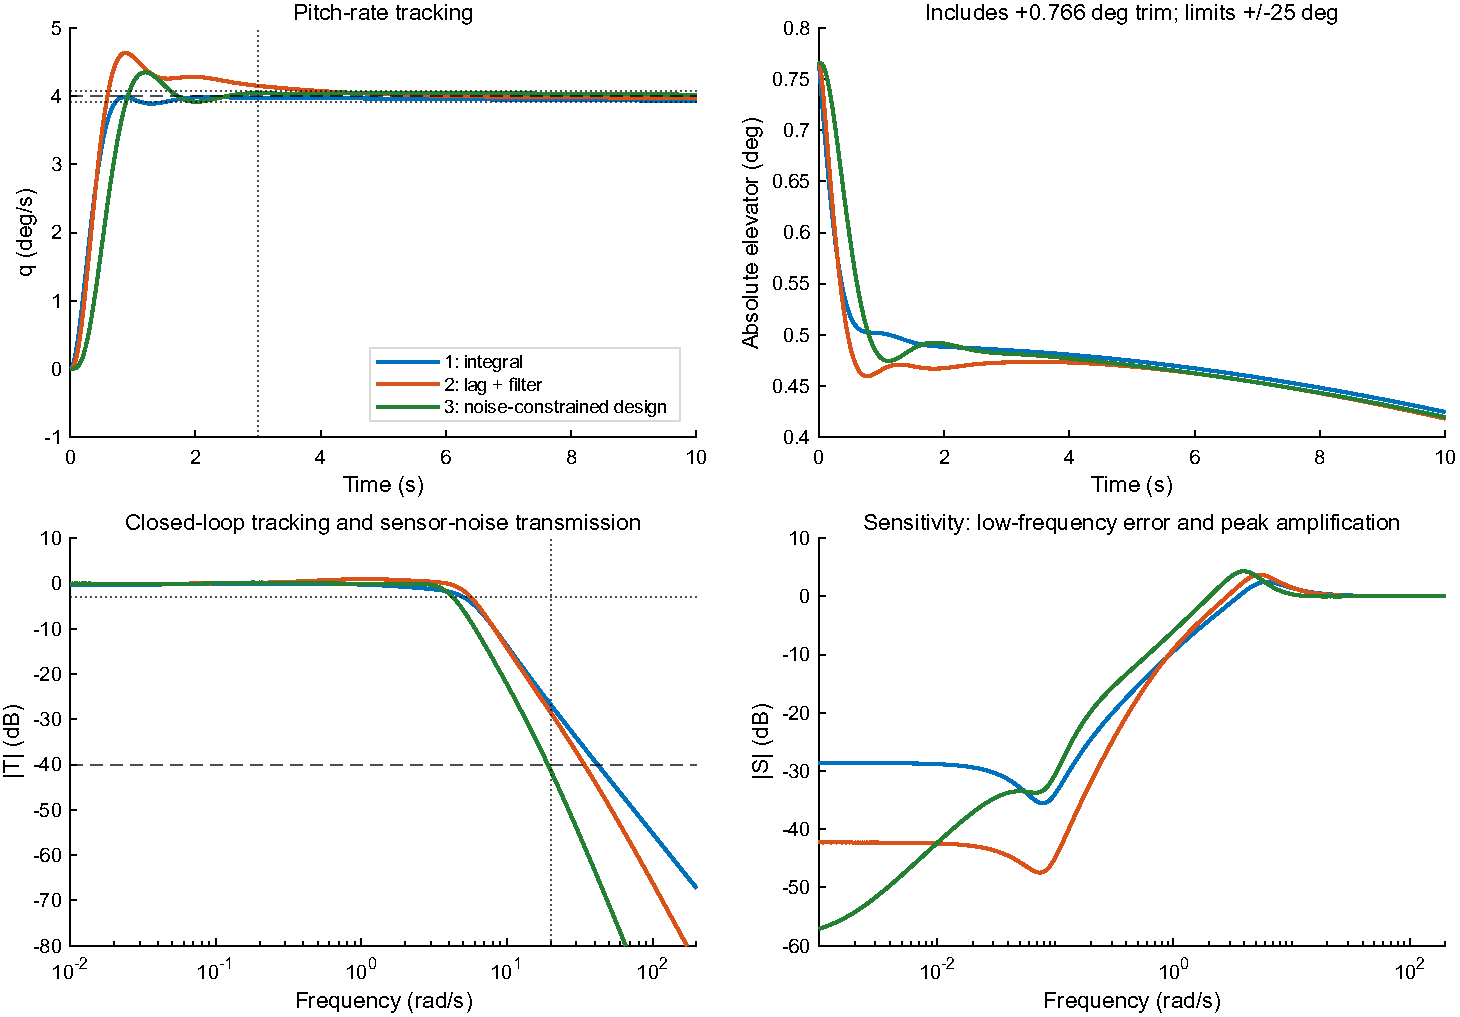
\includegraphics[width=1.0\linewidth]{comparison.pdf}\caption{角速度跟踪、绝对舵角、互补灵敏度与灵敏度对照。}\end{figure}


\clearpage\section{工程验证}
\subsection{空速}
在 180、210 节及 300 ft 下求解平飞迎角、油门和升降舵，再用中心差分重新线性化，控制器保持不变。油门位于 $[0,1]$，配平残差小于 $10^{-6}$。
\begin{table}[H]\centering\small\caption{同一控制器在独立验证配平点的表现。}
\begin{tabular}{lrrrrr}\toprule
Speed (kt) & Throttle & SSE (\%) & OS (\%) & $t_s$ (s) & $\omega_{BW}$\\\midrule
180 & 0.570 & 0.172 & 7.051 & 1.703 & 3.824\\
200 & 0.770 & 0.116 & 8.897 & 1.607 & 4.237\\
210 & 0.887 & 0.097 & 9.823 & 1.999 & 4.435\\
\bottomrule\end{tabular}\end{table}

三个离散测试点均满足主要时域与噪声指标。

\subsection{舵机与时延}
原始数据未提供舵机与传感器动态。舵机敏感性测试独立采用 $A_e(s)=1/(1+\tau s)$：
\begin{table}[H]\centering\small\caption{假设一阶舵机动态。}
\begin{tabular}{lrrrr}\toprule
$\tau$ (s) & SSE (\%) & OS (\%) & $t_s$ (s) & PM (deg)\\\midrule
0.000 & 0.116 & 8.897 & 1.607 & 60.301\\
0.025 & 0.116 & 12.377 & 2.275 & 57.460\\
0.050 & 0.116 & 15.878 & 2.451 & 54.738\\
0.100 & 0.116 & 22.314 & 3.757 & 49.748\\
\bottomrule\end{tabular}\end{table}

50 ms 工况满足主要阶跃指标；100 ms 工况的最小 q 通道稳定，但调节时间与超调超限。空速与舵机测试分开进行。

纯时延使相位裕度损失 $\omega_{gc}\tau_d$ 弧度，名义时延裕度约 0.522 s；10--40 ms 的结果见 \file{delay.csv}。非线性实现包含位置限幅和条件积分 [4]。当前测试均未触及位置及假设的 60 deg/s 舵速限制，饱和恢复性能仍待验证 [5]。

\subsection{参数扰动与数字实现}
俯仰刚度 $A_{32}$、阻尼 $A_{33}$ 和升降舵效能分别变化 $\pm20\%$，共 27 种组合。所有最小 q 通道稳定，其中 21 种满足全部时域指标，18 种满足噪声指标。超调范围 1.49--33.37\%，调节时间 1.07--3.28 s，相位裕度 39.00--73.41 度。

以 100 Hz 采样、飞机 ZOH、控制器 Tustin 离散化，最小闭环带宽为 4.258 rad/s，最大动态极点模为 0.999423949；未约简系统保留一个 $z=1$ 中性极点。实现时还需确定硬件延迟、量化、时钟抖动和抗混叠滤波。
\begin{figure}[H]\centering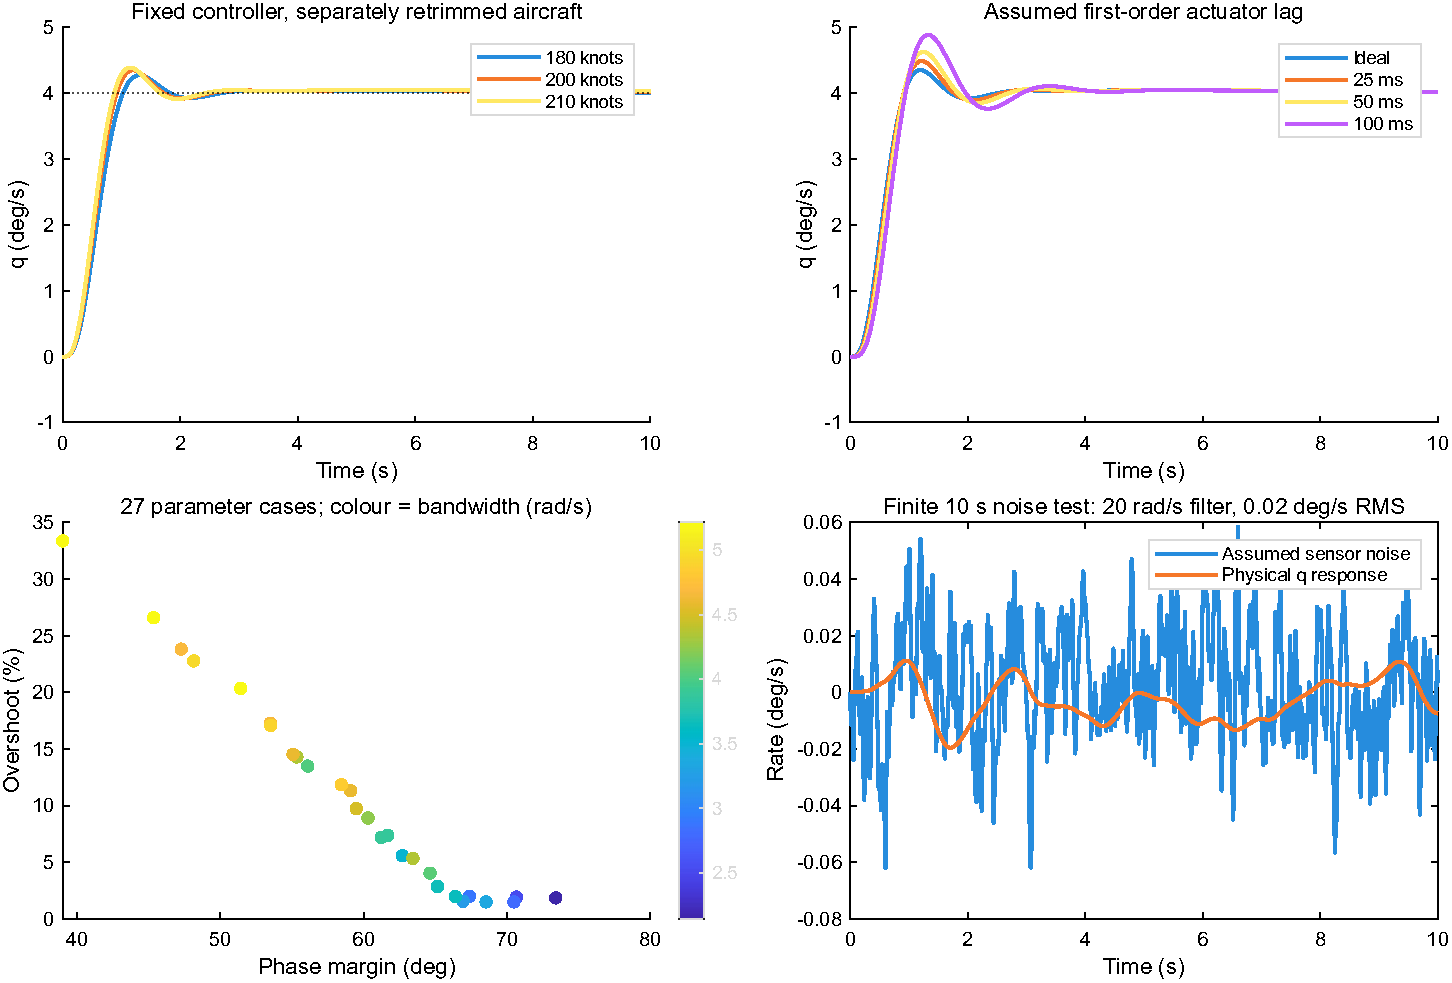
\includegraphics[width=1.0\linewidth]{robustness.pdf}\caption{分别进行的空速、舵机、参数扰动与有限记录噪声检查。}\end{figure}


\clearpage\section{非线性响应与内部动态}
未约简飞机与控制器系统含一个零特征值，其余特征值实部为负。由 $\dot\theta=q$，持续非零 q 产生俯仰角斜坡；$U=K_qS$ 的原点极点也使持续指令或传感器偏置引起控制漂移。外环需要管理姿态与指令。

采用原始十二状态非线性模型，并迭代收敛隐式气动导数。理想舵机 5 s 阶跃中，线性与非线性 q 最大差为 0.0403 deg/s。2 s 角速度脉冲的结果为：
\begin{itemize}
\item 峰值 q：4.3476 deg/s；最大绝对舵角：0.7732 度；最大舵速：0.478 deg/s。
\item 最大俯仰角：8.408 度；固定油门下最低速度：93.874 m/s。
\item 机体法向载荷峰值：1.759 g；线性与非线性 q 最大差：0.0314 deg/s。
\end{itemize}
200 节、4 deg/s 时 $Vq/g\approx0.73$，小舵角即可产生显著法向载荷。失速和结构裕度需要 $C_{L\max}$ 及载荷限制数据；速度损失说明后续需要自动油门。
\begin{figure}[H]\centering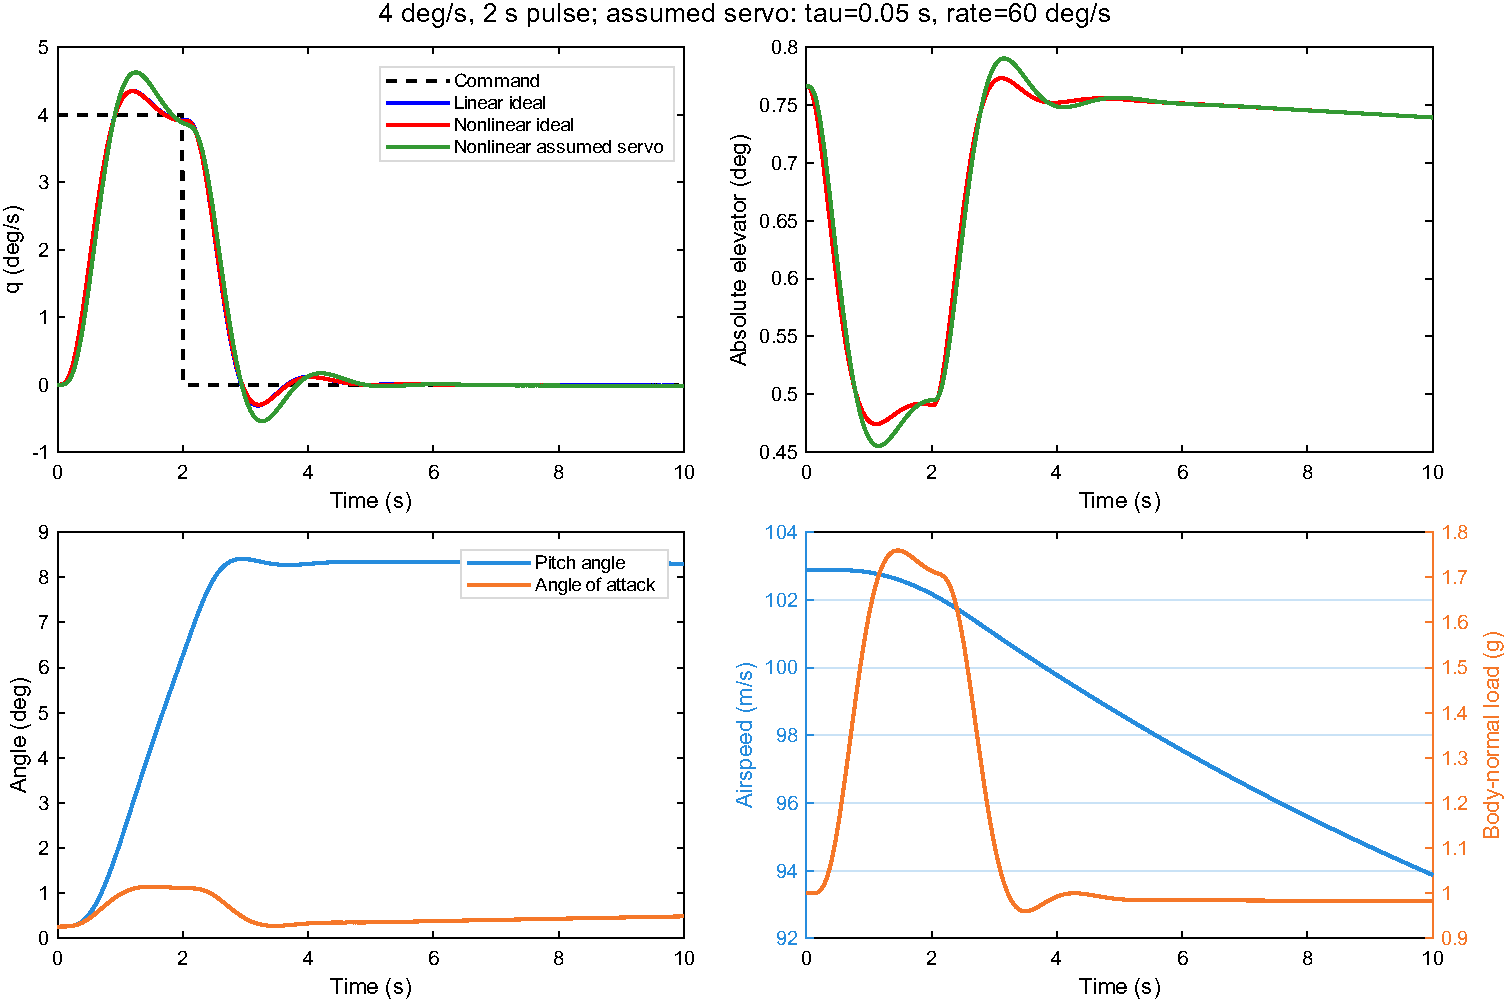
\includegraphics[width=1.0\linewidth]{nonlinear.pdf}\caption{有限角速度脉冲；假设舵机为 50 ms、60 deg/s。}\end{figure}


\subsection{测量噪声}
10 s 噪声测试采用假设的 0.02 deg/s RMS 测量噪声及 20 rad/s 低通。实际 q RMS 为 0.00804 deg/s，舵面增量 RMS 为 0.000547 度；名义 $|T(j20)|=-41.41$ dB。单侧等效面积 $\int_0^\infty|T/T(0)|^2d\omega$ 为 4.477 rad/s。舵面路径含积分器，其 RMS 仅适用于该有限记录。

\section{复现与后续工作}
从作业根目录运行：
\begin{verbatim}
run('inner_loop/run_inner.m')
open_sisotool(3)
\end{verbatim}
第一条命令重建控制器、验证结果、ZPK 和图表；第二条打开所选 SISOtool 模型。保留相邻 \file{Gqde}、\file{A_B_Matrix}、\file{trim} 文件夹。GUI 阶跃为归一化响应，数值测试以 rad/s 输入实际 4 deg/s 指令。

相关知识来自 Lecture 4--5（频响与模态）、8（根轨迹、裕度与补偿）、9（飞机控制结构与数字实现）、10（积分器配置、符号与 SCK）；Lecture 6--7、11 用于后续随机阵风分析。

下一步提取 $q_c\rightarrow V_s$，设计垂直速度外环、自动油门，并完成阵风分析与系统集成。

\section*{References / 参考资料}
\addcontentsline{toc}{section}{References / 参考资料}
\begin{enumerate}
\item MathWorks, \href{https://www.mathworks.com/help/control/ref/dynamicsystem.bandwidth.html}{bandwidth: frequency response bandwidth}.
\item MathWorks, \href{https://www.mathworks.com/help/control/ref/dynamicsystem.margin.html}{margin: gain/phase margins and crossover frequencies}.
\item MathWorks, \href{https://www.mathworks.com/help/control/ug/bode-diagram-design.html}{Bode diagram design}, and \href{https://www.mathworks.com/help/control/ref/controlsystemdesigner-app.html}{Control System Designer}.
\item MathWorks, \href{https://www.mathworks.com/help/simulink/slref/anti-windup-control-using-a-pid-controller.html}{Anti-windup control using PID Controller block}.
\item R. A. Hess and S. A. Snell, \href{https://ntrs.nasa.gov/citations/19980017538}{Flight Control System Design with Rate Saturating Actuators}, NASA/CR-97-207117, 1997.
\item AERO5560 Group Project, Longitudinal Task 1, pp. 2--3; Lectures 4, 5, 8, 9, 10 and 11, supplied course material. Aircraft data: Group 8 Canvas package.
\end{enumerate}
\end{document}
